% proposal.tex
\documentclass[12pt]{article}
\input{preamble}

\date{\today }

% author.tex
\author{
David J. Lilja\\
University of Minnesota\\
200 Union St. SE \\
4-174 Keller Hall \\
Minneapolis, MN 55455}


% title.tex
\title{Resource Management using Statistical Inference\\
 in Virtualized Environments}


\begin{document}

\bibliographystyle{plain}
\setcounter{page}{1}

\maketitle

%\input{checklist}

\newpage
%\pagestyle{empty}

% 1 page summary, required by NSF
% squinch space a bit if needed
% \setlength{\parindent}{0in}
% \setlength{\parskip}{0.5ex}
\section*{Project Summary {\small (1 page)}}
\addcontentsline{toc}{section}{A. Project Summary}
%
This is a three phase project. 
The first phase is to predict the performance of a virtual disk given a workload and a storage system. 
The second phase is to model the performance interference between different virtual disks on a single storage system. 
The last phase is to map application requirements to resource mapping.

The first phase will result in virtual disk performance model. 
In our previous work with VMware, we developed a storage performance modeling framework called Romano. 
This differs from previous model, Pesto\cite{pesto}, currently in use by \emph{Virtual Center} product in that it identifies the key characteristics of workload that affects the performance (using ANOVA\cite{lilja}).
The resulting accuracy is improved by 80\% allowing much more aggressive load balancing. 
\begin{figure}[t!]
\centering
\subfloat[Pesto]{\label{rdPesto}\includegraphics[width=0.4\columnwidth, clip, trim=0 0.5in 0.2in 0.7in]{error_hist_compare_pesto.pdf}}
\subfloat[Romano]{\label{rdRomano}\includegraphics[width=0.4\columnwidth, clip, trim=0 0.5in 0.2in 0.7in]{error_hist_compare_kromano.pdf}}
\caption{Distribution of residuals($\epsilon$) for Pesto and Romano.
x-axis is the value of $\epsilon$ in $ms$.
y-axis is number of occurrences+1.
Addition of 1 was required to allow y-axis to be in log scale.
%The $\epsilon$ distribution does not changes widely for Romano indicating that the accuracy of Romano is less data store dependent. 
%Furthermore, Romano's $\epsilon$ are symmetric around 0, indicating that residuals are unbiased.
}
\label{residualDist}
\end{figure}
The residuals from both techniques are shown in Figure \ref{residualDist} for four different storage systems.
While this approach is very good at predicting a data store performance, it currently lacks the ability to predict the performance for each virtual disk when they are consolidated onto a single data store. 

In the second phase, we will apply statstical inference on the effect of interference, we plan to derive each VM's IO performance without having to actually change the system state.  
This allows IT administrators to simulate their configuration changes in the large scale data centers without disrupting their operation. 

The last phase will allowing application level performance requirements to be mapped to VM level configurations, users can simply specify the desired behavior without having to worry about the VMware product details.


%\newpage
\pagestyle{plain}
\setcounter{page}{1}

% GPG dictates section, so must use \subsection inside
\section*{Project Description}  %% limited to 15 pages 
\addcontentsline{toc}{section}{C. Project Description}

%% {\em The main body of the proposal should be a clear statement of
%% the work to be undertaken and should include: objectives for the
%% period of the proposed work and expected significance, relation to
%% longer-term goals of the PI's project, and relation to the present
%% state of knowledge in the field, to work in progress by the PI
%% under other support and to work in progress elsewhere.  The
%% statement should outline the general plan of work, including 
%% the broad design of activities to be undertaken, an adequate
%% description of experimental methods and procedures, and if
%% appropriate, plans for preservation, documentation, and sharing of
%% data, samples, physical collections and other related research
%% products.  Any substantial collaboration with individuals not
%% included in the budget should be described with a letter from 
%% each \ldots.} 

% a top-level Section, with Subsections
% objectives.tex
\section{Research Objectives}
\label{objectives}
%
The objective of this project is to automatically map a given application requirements to physical hardware resources such that the application performance can be maintained in a highly consolidated environments. 

The virtualization layer will provide the framework to partition the available hardware resources and to isolate the performance interference between them\cite{}. 
The management layer will provide means to create a \emph{pool} of resources from cluster of heterogenous machines\cite{}, increasing the total amount of resources available for mapping. 
Live migration techniques\cite{} allow applications to be remaped based on the time varying demands and machine availbility. 
These mechanisms already exists in current virtulization infrastructure.
However, the mapping itself is still carried out manually decreasing the benefits of virtualization and explosing the system to the human error. 

To achieve our objective, the system must be aware of the workload changes, remap the resources and ensure that remaping satisfies the requirements all active applications.
A significant progress has already been made to migrate virtual machines to load balance CPU and memory resources\cite{}.
However, correct IO performance prediction is a much harder problem due to the statefulness of the storage systems\cite{}.
Another problem is that virtualization fails to isolate the performance interference of consolidated IO workloads as well as it isolates the CPU, memory and network resources. 
Last problem is lack of mapping between the application requirements and the virtualized resources. 
The actual application requirements are typically not specified interms of resource usage. 
Instead they are typically determined by the end user demand it must satisfy.   
A mechanism to monitor and model the application performance behavor is the last requirement of this project. 


\subsection{Intellectual Merit of the Proposed Work}
%
Describe the intellectual merit of the proposed work here.

\begin{figure}[h]
\centerline{\mbox{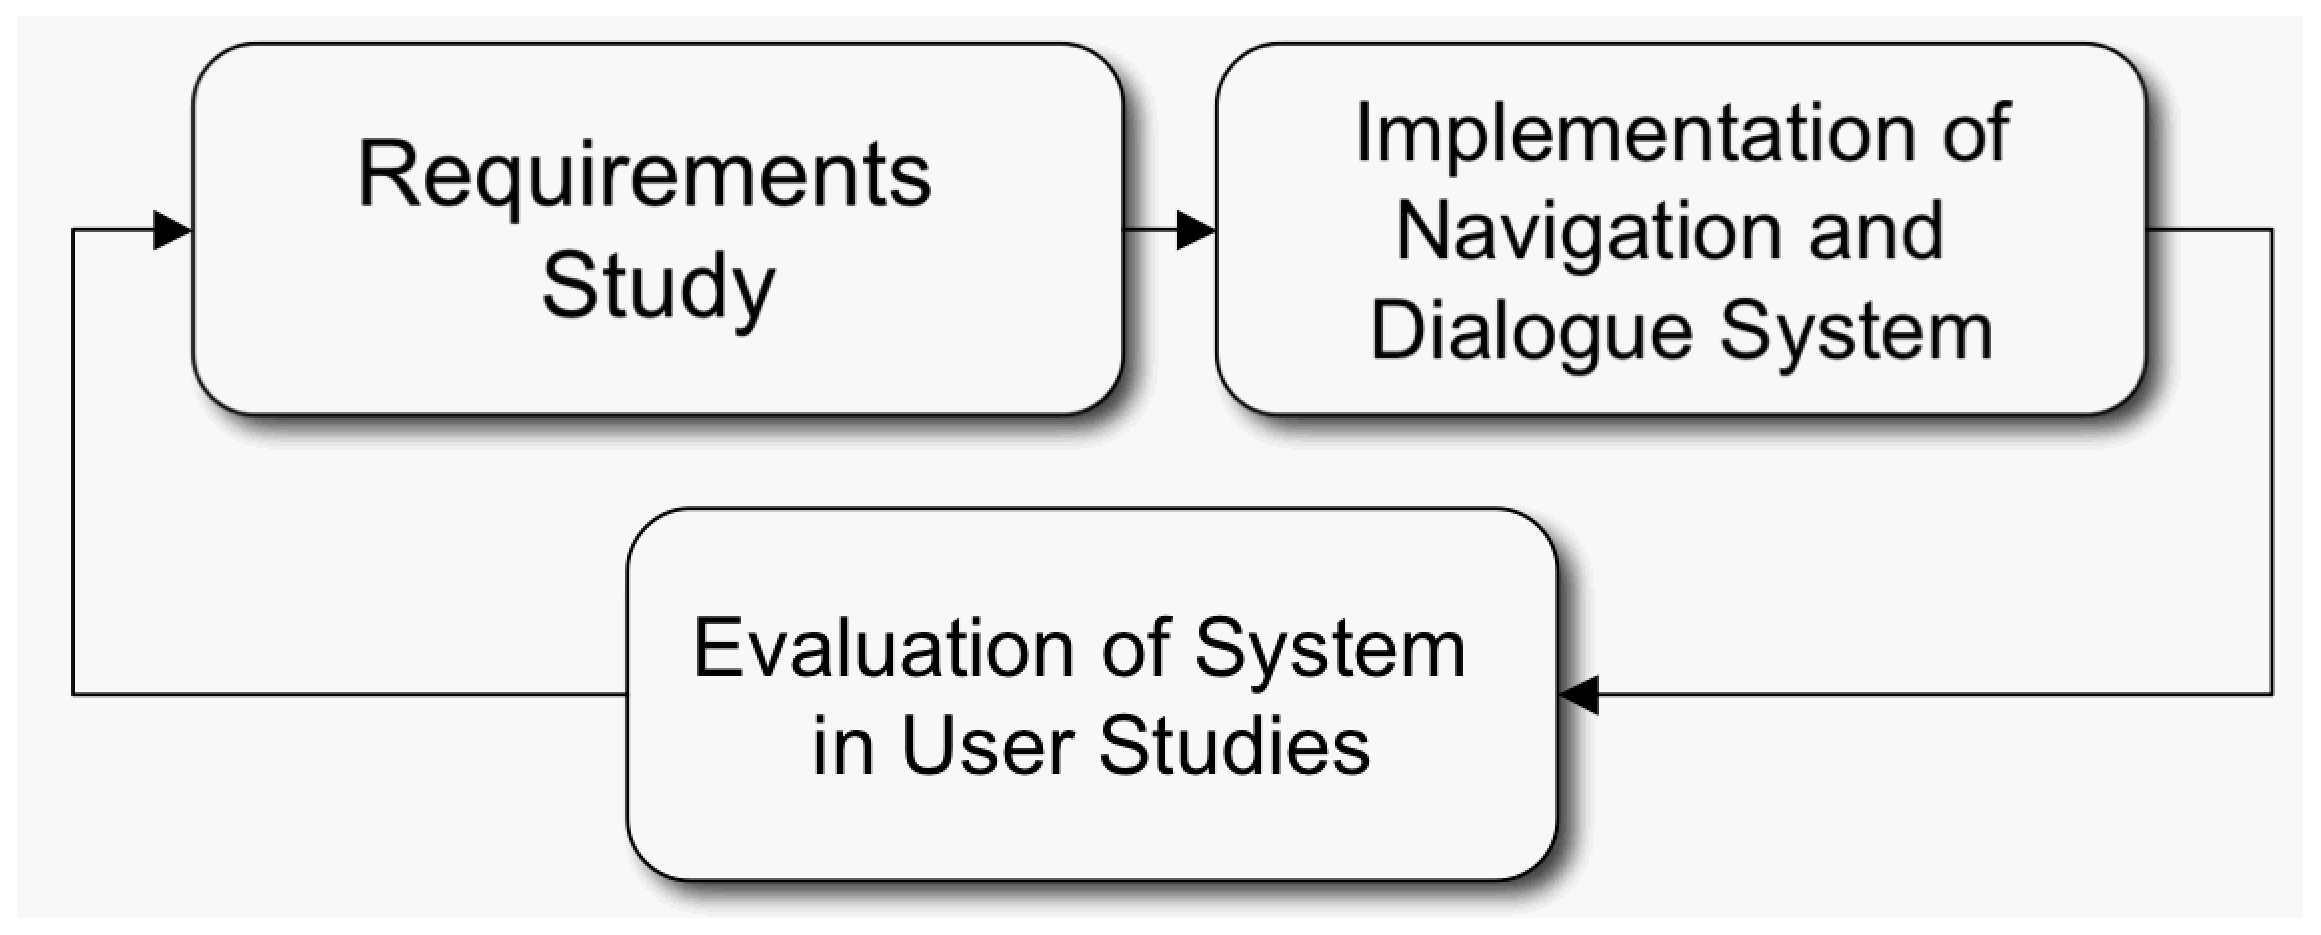
\includegraphics[width=3in]{cycle}}}
\caption{Our proposed research plan involves an iterated 
         cycle of design, implementation and user testing.}
\label{fig:cycle}
\end{figure}

Describe the intellectual merit of the proposed work here.

\subsection{Impact on VMware}
%
Describe the broader impact of the proposed work here.

Describe the broader impact of the proposed work here.


% more technical content
\input{architecture}

% statement of work
% plan.tex
\section{Statement of Work}
\label{plan}
%
This is a three phase project. The first phase is to predict the performance of a virtual disk given a workload and a storage system. The second phase is to model the performance interference between different virtual disks on a single storage system. The last phase is to map application requirements to resource mapping. 

\subsection{Schedule}
%
\bigskip
\begin{tabular}{l|l}
\hspace{.25in} Year 1 \hspace{.25in} & 
\begin{minipage}{5in}
  Virtual Disk Performance Model\\
	Workload Interference Model\\
  \\
  By the end of year 1, we expect to determine pseudo-optimal virtual disk placements such that performance requirement of each virtual disk is satisfied with minimum number of storage systems.
\medskip
\end{minipage}\\
\hline
\hspace{.25in} Year 2 & 
\begin{minipage}{5in}
  \medskip
  Application Performance Monitor\\
	Dynamic Resource Allocator\\
  \\
  By the end of year 2, we expect to meet the various application requirements by dynamically mapping of resources and performing necessary migrations. 
\medskip
\end{minipage}\\
\end{tabular}

\subsection{Deliverable} 
\label{deliverable} 
%
\begin{itemize}
\item Fully functional system that monitors application behaviors as well as VM behaviors to map available resources on heterogenous compute and storage nodesto satisfy the diverse requirements of IO intensive applications. 
\item Statsitical models that allow IO performance prediction at virtual disk level. 
\end{itemize}


% related work
%% significance.tex
\section{Related Work}
%
Describe related work \cite{bar,foo} here.


% prior NSF work by PI's
%\input{priornsf}

% turn off pagination; no page limit for references
\pagestyle{empty}
\renewcommand{\refname}{References Cited}
% generate References Cited section
\bibliography{refsA}

%\newpage

% description of facilities
%\input{facilities}

\newpage

% budget justification
%% budget.tex
% defs for below.  note " " after defs.
\def\piA{David J. Lilja}
\def\numRAs{2}
\def\pilist{PI: \piA}
\def\thisyear{2012}
\def\startdate{09/02/2012}
\def\enddate{09/01/2012}
\def\phdstipend{\$2,125/mo }
\def\mscstipend{\$1,940/mo }
\def\studraise{4\% }
\def\salaryallocationrate{8.34\%} % no trailing space
\def\employeebenefitrate{27.0\% }
\def\vacationaccrualrate{9.5\% }
\def\networkservicescost{\$100/person/month }
\def\networkfacilitycharges{\$150/person/month} % no trailing space
\def\MITninemonthtuition{\$33,400} % no trailing space
\def\MITtuitioninflator{4\% }
\def\MITtuitionsubsidy{45\% }
\def\MITtuitioncharge{55\% }
\def\msAllocation{1.24\%}
\def\facostinception{07/01/2006} % no trailing space
\def\facostrate{65\% }

% make the outer enumerated list alpha A, B, C ...
\renewcommand{\theenumi}{\Alph{enumi}}
\renewcommand{\theenumii}{\arabic{enumii}}

\vspace*{1.0in}
\begin{center}
{\large
UMN / ARTiC Laboratory \\
\pilist \\
Proposed Budget Period: \startdate -- \enddate \\
Budget Justification for Cost Proposal
}
\end{center}

\begin{enumerate}

%A
\item \underline{Key Personnel:}

\begin{tabular}{|l|l|} \hline
\underline{Last Name} & \underline{Review/Raise} \\ \hline
\piA & June \\ \hline
\end{tabular}

MIT fully supports the academic year salaries of professors, associate
professors, and assistant professors, but makes no specific commitment
of time or salary to any individual research project.

%B
\item \underline{Other Personnel:}

\begin{enumerate}
  \item \underline{Research Assistants:} \\{~}\\
100\% of the stipend is charged to the research project. The RA stipend
is not subject to employee benefits. Stipend for the year beginning on
\startdate is \phdstipend for a PhD student and \mscstipend for a
Masters student. A \studraise raise is applied each year (in June).

%2
  \item \underline{Other (Technical \& Administrative Support):}\\{~}\\
The Computer Science Artificial Intelligence Laboratory (CSAIL) provides administrative
services for all principal investigators who submit proposals through CSAIL. These
administrative services are run by the Headquarters Staff and include Fiscal, Personnel,
Facilities and other CSAIL operations.\\{~}\\
These services are supported by an Allocated Project Level Cost, which is assessed against all
contracts and grants. The current rate for the Salary Allocation is \salaryallocationrate. The Allocation
Base is shown below:

\begin{tabular}{|c|c|c|c|} \hline
Allocation & Year 1 & Year 2 & Year 3 \\ \hline
Base & \$XXX,YYY & \$XXX,YYY & \$XXX,YYY \\ \hline
\end{tabular}

\end{enumerate}

\item \underline{Fringe Benefits}

\begin{enumerate}

%(a)
\item Employee benefits are calculated at the rate of \employeebenefitrate and 
are applied to total salary expenses, less Research Assistants.

\item Vacation accruals are calculated at the rate of \vacationaccrualrate and 
are applied to total salary expenses, less Faculty and Research
Assistants.

\end{enumerate}

%D
\item \underline{Travel:}

\begin{enumerate}

\item \underline{Domestic Travel:}

\item \underline{Foreign Travel:}

\end{enumerate}

\item \underline{Other Direct Costs:}

\begin{enumerate}

\item \underline{Material \& Supplies:}\\{~}\\
Estimated costs for software and supplies needed for the project.

\item \underline{Computer Services:}\\{~}\\
MIT/CSAIL has a centralized network services function. The costs consist of Network Services at
\networkservicescost and Network Facility Charges at \networkfacilitycharges. The base number of
people used for this calculation was \numRAs (the two full time RAs).

\item \underline{Other:}\\{~}\\
(a) RA tuition: For the academic year starting \thisyear, MIT 9-month
tuition is \MITninemonthtuition. A \MITtuitioninflator annual inflator
is applied each year. MIT will subsidize \MITtuitionsubsidy of tuition,
leaving \MITtuitioncharge to be charged to the project. During the
summer, MIT has waived tuition.\\{~}\\ 
(b) Allocated expenses are assessed against all contracts and
grants. The current rate for the Materials and Services Allocation is
\msAllocation. These funds help support the Headquarters staff mentioned
above in the section entitled ``Other (Technical \& Administrative
Support)''. Please see the table in that section for the allocation
base.

\item \underline{Equipment:}

The equipment line items will support purchases as follows:

\begin{itemize}

\item Year One (\$X,XXX): enter purpose, items and costs here

\item Year Two (\$X,XXX): enter purpose, items and costs here

\item Year Three (\$X,XXX): enter purpose, items and costs here

\end{itemize}

\item \underline{[Describe any other direct cost items here]:}

\end{enumerate}

\item \underline{Indirect Costs (Facilities \& Administrative Costs):}\\{~}\\
Effective \facostinception, F\&A Costs are calculated by applying the
negotiated rate of \facostrate to the Modified Total Direct Cost (MTDC)
base. The MTDC base includes all direct costs, except Graduate Student
Tuition, Network Facilities Charges, the Salary Allocation (and
associated benefits), and the Materials and Services Allocation.

\end{enumerate}


%\newpage

% bios for all Co-PI's (not required for Co-I's)
\section*{PI Biography: Person A}
%
{\nibf{Professional Preparation:}}
%
\begin{verbatim}
School                              Degree                     Date
\end{verbatim}

\nibf{Appointments}

\begin{verbatim}
Organization                        Position                   Date
\end{verbatim}

\nibf{Publications Relevant to Proposal}

\begin{verbatim}
1. Authors,
   Title,
   Booktitle,
   Location, Month, Year, Pages.
2. Authors,
   Title,
   Venue,
   Location, Month, Year, Pages.
\end{verbatim}

\nibf{Other Selected Publications}

\begin{verbatim}
1. Authors,
   Title,
   Booktitle,
   Location, Month, Year, Pages.
2. Authors,
   Title,
   Booktitle,
   Location, Month, Year, Pages.
\end{verbatim}

\nibf{Synergistic Activities}

\begin{verbatim}
1. Activity 1.
2. Activity 2.
\end{verbatim}



\end{document}
